\chapter{Numeryczne metody estymacji}\label{numPAJ}

Przez numerykę rozumie się dziedzinę matematyki
zajmującą się przybliżonym rozwiązywaniem zagadnień algebraicznych. Odkąd zjawiska przyrodnicze zaczęto opisywać przy użyciu formalizmu matematycznego,
pojawiła się potrzeba rozwiązywania zadań analizy matematycznej czy algebry. Dopóki były
one nieskomplikowane, dawały się rozwiązywać analitycznie, tzn. z użyciem pewnych
przekształceń algebraicznych prowadzących do otrzymywania rozwiązań. Z czasem jednak, przy powstawaniu coraz to bardziej skomplikowanych teorii
opisujących zjawiska, problemy te stawały się na tyle złożone, iż ich rozwiązywanie ścisłe
było albo bardzo czasochłonne albo też zgoła niemożliwe. Numeryka pozwalała znajdywać
przybliżone rozwiązania z żądaną dokładnością. Ich podstawową zaletą była ogólność tak
formułowanych algorytmów, tzn. w ramach danego zagadnienia nie miało znaczenia czy było
ono proste czy też bardzo skomplikowane (najwyżej wiązało się z większym nakładem pracy
obliczeniowej). Natomiast wadą była czasochłonność. Stąd prawdziwy renesans metod
numerycznych nastąpił wraz z powszechnym użyciem w pracy naukowej maszyn cyfrowych,
a w szczególności komputerów \cite{milewski}. 

Dziś dziesiątki żmudnych dla człowieka operacji
arytmetycznych wykonuje komputer, jednak złożoność obliczeniowa algorytmów uczących i modeli statystycznych stała się krytycznym czynnikiem ograniczającym w sytuacjach, gdy rozważane są duże zbiory danych. Te ograniczenia spowodowały, że w uczeniu maszynowym i modelowaniu statystycznym wielkiej skali zaczęto wykorzystywać algorytmy \textbf{stochastycznego spadku gradientu}. 

W poniższym rozdziale przedstawione są klasyczne algorytmy spadku wzdłuż gradientu Cauchy'ego oraz Raphsona-Newtona. Następnie omówiony jest algorytm stochastycznego spadku wzdłuż gradientu, którego wykorzystanie do estymacji współczynników w modelu Coxa jest kluczowym celem tej pracy. Algorytm stochastycznego spadku gradientu to metoda optymalizacji wzdłuż spadku gradientu wykorzystywana w sytuacjach, gdy rozważaną funkcję można zapisać jako sumę różniczkowalnych składników. Ponieważ popularne metody statystycznej estymacji takie jak algorytm Fishera (\textit{ang. Fisher scoring}, \cite{fisher3}), algorytm EM (\textit{ang. Expectation–maximization algorithm}, \cite{dempster}) czy iteracyjna ważona metoda najmniejszych kwadratów (\cite{greenPJ}) nie zawsze przenoszą się na zastosowania do danych dużej skali bądź danych napływających (\textit{ang. streaming data}), niekiedy algorytm stochastycznego spadku gradientu jest jedyną dostępną metodą optymalizacji numerycznej. Ponadto przedstawiono również zalety algorytmów stochastycznego spadku gradientu, które przemawiają za atrakcyjnością i popularnością tego typu rozwiązania. 

Definicje i pojęcia w tym rozdziale pochodzą z~\cite{bott1},~\cite{bott2},~\cite{kotlowski}~i~\cite{fortuna}.

\newpage
\section{Algorytmy spadku wzdłuż gradientu}\label{R-N}

Poniższy rozdział przedstawia popularne iteracyjne algorytmy wyznaczania przybliżonej wartości miejsca zerowego funkcji oraz rozważaną w pracy metodę stochastycznego spadku gradientu. Szukanie miejsc zerowych funkcji jest przydatne w problemach optymalizacyjnych, gdy celem jest znalezienie pierwiastka pochodnych badanej funkcji. Dodatkowo takie algorytmy wykorzystywane są do rozwiązywania (nieliniowych) układów równań. Metody iteracyjne składają się zazwyczaj z $k$ kroków bądź są zatrzymywane, gdy osiągnięty zostanie warunek stopu, czyli gdy odległość pomiędzy kolejnymi przybliżeniami jest dość mała $\parallel w_{k+1}-w_k\parallel < \varepsilon$ lub wartość gradientu funkcji w wyznaczonym punkcie jest bliska wektorowymi zerowemu $\parallel \nabla_Q(\mathbf{w_k}) \parallel \leqslant \varepsilon$ (test stacjonarności), gdzie $\varepsilon$ to zadana z góry precyzja.
Metoda stochastycznego spadku wzdłuż gradientu zakłada, że minimalizowaną funkcję $Q(w)$ można przedstawić jako różniczkowalną sumę jej składników $Q(w) = \sum_{i=1}^{n}Q_i(w)$. W~poniższych algorytmach $\alpha_k$ oznacza długość kroku algorytmu.
\begin{center}
\textbf{Metoda spadku wzdłuż gradientu I (Cauchy’ego)}
\end{center}
Minimalizacja funkcji $Q(w)$:
\begin{itemize}
\item Zaczynamy od wybranego rozwiązania startowego, np. $w_{0} = 0$.
\item Dla $k = 1, 2, \dots$ aż do zbieżności
	\begin{itemize}
	\item Wyznaczamy gradient w punkcie $w_{k-1}, \nabla_{Q}(w_{k-1})$.
	\item Robimy krok wzdłuż negatywnego gradientu: $$w_{k} = w_{k-1} - \alpha_{k}\nabla_{Q}(w_{k-1}). $$
	\end{itemize}
\end{itemize}

\begin{center}
\textbf{Metoda spadku wzdłuż gradientu II (Newtona-Raphsona)}
\end{center}
Minimalizacja funkcji $Q(w)$:
\begin{itemize}
\item Zaczynamy od wybranego rozwiązania startowego, np. $w_{0} = 0$.
\item Dla $k = 1, 2, \dots$ aż do zbieżności
	\begin{itemize}
	\item Wyznaczamy~gradient~w~punkcie~$w_{k-1}, \nabla_{Q}(w_{k-1})$~i~odwrotność~$(D_{Q}^{2}(w_{k-1}))^{-1}$.
	\item Robimy krok wzdłuż negatywnego gradientu z zadanym krokiem przez Hesjan: 
	\begin{equation}\label{NJU-rap}
	 w_{k} = w_{k-1} - (D_{Q}^{2}(w_{k-1}))^{-1}\nabla_{Q}(w_{k-1}). 
	 \end{equation}	
	\end{itemize}
\end{itemize}
\begin{center}
\textbf{Metoda stochastycznego spadku wzdłuż gradientu I}
\end{center}
Minimalizacja funkcji $Q(w)$:
\begin{itemize}
\item Zaczynamy od wybranego rozwiązania startowego, np. $w_{0} = 0$.
\item Dla $k = 1, 2, \dots$ aż do zbieżności
	\begin{itemize}
	\item Wylosuj $i \in \{1,\dots,n\}$
	\item Wyznaczamy gradient funkcji $Q_{i}$ w punkcie $w_{k-1}, \nabla_{Q_{i}}(w_{k-1})$.
	\item Robimy krok wzdłuż negatywnego gradientu: 
	\begin{equation}\label{sgdrownanie}
	 w_{k} = w_{k-1} - \alpha_{k}\nabla_{Q_{i}}(w_{k-1}).
	  \end{equation}
	\end{itemize}
\end{itemize}

\section{Algorytm stochastycznego spadku wzdłuż gradientu I}\label{SGD}
Stochastyczny spadek gradientu to popularny algorytm wykorzystywany do estymacji współczynników w szerokiej gamie modeli uczenia maszynowego takich jak maszyny wektorów podpierających (\textit{ang. Support Vector Machines}), regresja logistyczna czy modele graficzne~\cite{finkel}. W~połączeniu z algorytmem propagacji wstecznej jest standardowym algorytmem w~trenowaniu sztucznych sieci neuronowych. Algorytm stochastycznego spadku gradientu był używany już od 1960 przy estymacji współczynników w modelu regresji liniowej, oryginalnie znanym jako \textit{ADALINE} \cite{ADALINE}. Kolejnym algorytmem wykorzystującym stochastyczny spadek gradientu jest filtr adaptacyjny najmniejszych średnich kwadratów \cite{widrow2} (\textit{ang.~least mean squares (LMS) adaptive filter}), który został wynaleziony przez Bernarda Widrowa, twórcę \textit{ADALINE}.

Idea algorytmu stochastycznego spadku gradientu jest następująca: zamiast obliczać gradient na całej funkcji $L$, w danym kroku oblicz
gradient tylko na pojedynczym elemencie $\ell_{i}$. Nazwa \textit{stochastyczny} bierze się stąd, iż oryginalnie wybiera
się element $\ell_{i}$ losowo. W praktyce zwykle przechodzi się po całym zbiorze danych w losowej kolejności.

\subsubsection{Właściwości stochastycznego spadku wzdłuż gradientu}

Zbieżność algorytmu stochastycznego spadku gradientu była szeroko badana w literaturze aproksymacji stochastycznych. Aby uzyskać zbieżność zazwyczaj wymaga się aby ciąg kroków algorytmu $\alpha_k$ był malejący i spełniał poniższe warunki $\sum\nolimits_k \alpha_k = \infty$ oraz $\sum\nolimits_k \alpha_k^2 < \infty$~\cite{bott1}.
Twierdzenie Robbinsa-Siegmunda \cite{robbins} przy łagodnych warunkach zapewnia~zbieżność~prawie na pewno \cite{bottDOD}, nawet  gdy~optymalizowana~funkcja~nie~jest~wszędzie~różniczkowalna.

Prędkość zbieżności stochastycznego spadku gradientu jest w rzeczywistości ograniczana przez zgrubną (\textit{ang. noisy}) aproksymacje prawdziwego gradientu. Gdy długości kroków algorytmu
maleją zbyt wolno, wariancja estymatorów parametrów $w_k$ maleje równie wolno. Gdy kroki algorytmu maleją
zbyt szybko, oczekiwane estymatory parametrów $w_k$ potrzebują więcej czasu by osiągnąć optimum \cite{bott1}. Pod pewnymi warunkami regularności \cite{murata}, najlepsza prędkość zbieżności jest uzyskana dla kroków algorytmu $\alpha_k\sim k^{-1}$.

Jak wykazano w \cite{dennis} pod pewnymi odpowiednimi warunkami regularności, gdy zainicjowany współczynnik początkowy $w_0$ jest wystarczająco blisko optimum i krok algorytmu jest odpowiednio mały, algorytm stochastycznego spadku gradientu osiąga liniową zbieżność. Oznacza to, iż przy spełnieniu założeń metody, odległości pomiędzy kolejnymi przybliżeniami a minimum funkcji $\mathbf{w^{\ast}}$ maleją liniowo: $\parallel \mathbf{w^{\ast}} - \mathbf{w_{k+1}} \parallel \leqslant c \parallel \mathbf{w^{\ast}} - \mathbf{w_k} \parallel$. Zbieżność wymaga często przejścia parokrotnie po całym
zbiorze danych. Wady i zalety algorytmu wymienione są poniżej. Zalety~zdecydowanie przewyższają~wady.

\textbf{Zalety} \vspace{-5pt}
\begin{itemize}
\item \textcolor{orange}{Szybkość kroku}: obliczenie gradientu wymaga wzięcia tylko jednej
obserwacji.
\item \textcolor{orange}{Skalowalność}: cały zbiór danych nie musi nawet znajdować się
w pamięci operacyjnej.
\item \textcolor{orange}{Prostota}: gradient funkcji  $Q_{i}$ daje bardzo prosty wzór na
modyfikacje wag.
\end{itemize}

\textbf{Wady}  \vspace{-5pt}
\begin{itemize}
\item \textcolor{orange}{Wolna zbieżność}: czasem gradient stochastyczny do zbieżności wymaga wielu iteracji po zbiorze uczącym.
\item \textcolor{orange}{Problem z ustaleniem długości kroku $k$}: wyznaczenie $k$
przez przeszukiwanie liniowe nie przynosi dobrych rezultatów,
ponieważ nie optymalizujemy oryginalnej funkcji $Q$ tylko jej jeden
składnik $Q_{i}$.
\end{itemize}
\newpage
\section{Porównanie algorytmów spadku wzdłuż gradientu}

W niniejszym podrozdziale przedstawiono graficznie różnice w wyborze kolejnych punktów w trakcie optymalizacji między omawianymi w poprzedniej części pracy algorytmami spadku wzdłuż gradientu I (Cauchy'ego), spadku wzdłuż gradientu II (Newtona-Raphsona) oraz stochastycznego spadku wzdłuż gradientu I. W celu zobrazowania przykładu na dwuwymiarowym wykresie, postanowiono ograniczyć się do modelu z jedną zmienną objaśniającą i wyrazem wolnym. Do przykładu wybrano model regresji logistycznej, z racji na prostotę przedstawienia funkcji log-wiarogodności jako sumy różniczkowalnych składników.

Funkcja log-wiarogodności dla modelu regresji logistycznej, za \cite{czepiel} i \cite{dobson}, ma postać

\begin{equation}\label{logglm}
\marginnote{$\beta=(\beta_1,\beta_2)$}
\ell(\beta) =: \sum\limits_{i=1}^{N} Q_i(\beta_1,\beta_2), 
\end{equation}
\begin{equation}
Q_i(\beta_1,\beta_2) = y_i(\beta_1+\beta_2x_i) -\log(1+\exp(\beta_1+\beta_2x_i)).
\end{equation}

Dla tak skonstruowanej funkcji wiarogodności, współrzędne gradientu to odpowiednio

\begin{equation*}
\dfrac{\partial\ell(\beta)}{\partial\beta_1} = \sum\limits_{i=1}^{N}\Big(y_i-\pi_i(\beta)\Big), \ \ \
\dfrac{\partial\ell(\beta)}{\partial\beta_2} = \sum\limits_{i=1}^{N}x_i\Big(y_i-\pi_i(\beta)\Big), \ \ \
\pi_i(\beta) = \frac{\exp(\beta_1+\beta_2x_i)}{1+\exp(\beta_1+\beta_2x_i)},
\end{equation*}

zaś macierz informacji wyraża się jak następuje
\begin{equation}\label{iii}
\mathscr{I}(\beta) = 
\begin{bmatrix}
    \sum\limits_{i=1}^{N}\pi_i(\beta)(1-\pi_i(\beta))       & \sum\limits_{i=1}^{N}x_i\pi_i(\beta)(1-\pi_i(\beta)) \\
\sum\limits_{i=1}^{N}x_i\pi_i(\beta)(1-\pi_i(\beta)) & \sum\limits_{i=1}^{N}x_i^2\pi_i(\beta)(1-\pi_i(\beta)) 
\end{bmatrix},
\end{equation}
gdzie $N$ to liczba obserwacji.

Wtedy aktualizacja kandydata na miejsce zerowe w $k$-tym kroku algorytmu optymalizacyjnego dla kolejnych metod omówionych w rozdziale (\ref{R-N}) wyraża się poniższymi wzorami
\\
\begin{center}
\textbf{Metoda spadku wzdłuż gradientu I (Cauchy’ego)}
\end{center}
\begin{equation*}
\beta_{k} = \beta_{k-1} + \alpha_{k}\cdot\Big(\sum\limits_{i=1}^{N}(y_i-\pi_i(\beta_{k-1})), \sum\limits_{i=1}^{N}x_i(y_i-\pi_i(\beta_{k-1}))\Big).\marginnote{$\alpha_k \in \mathbb{R}$}
\end{equation*}
\begin{center}
\textbf{Metoda spadku wzdłuż gradientu II (Newtona-Raphsona)}
\end{center}
\begin{equation*}
\beta_{k} = \beta_{k-1} + \mathscr{I}(\beta_{k-1})^{-1}\cdot\Big(\sum\limits_{i=1}^{N}(y_i-\pi_i(\beta_{k-1})), \sum\limits_{i=1}^{N}x_i(y_i-\pi_i(\beta_{k-1}))\Big),
\end{equation*}
gdzie $\mathscr{I}(\beta_{k-1})$ zdefiniowane jest we wzorze (\ref{iii}). 
\begin{center}
\textbf{Metoda stochastycznego spadku wzdłuż gradientu I}
\end{center}
\begin{equation*}
\beta_{k} = \beta_{k-1} + \alpha_{k}\cdot\Big(y_i-\pi_i(\beta_{k-1}), x_i(y_i-\pi_i(\beta_{k-1}))\Big),
\end{equation*}
dla wylosowanego w danym kroku $i$.
\\ \ \\
Ponieważ algorytmy te znajdują minimum funkcji, a docelowo szukane jest maksimum, stąd wykorzystano przeciwieństwo funkcji log-wiarogodności, dlatego w wyżej wymienionych wzorach zmieniono znaki przed pochodnymi na przeciwne.

\newpage
\subsubsection{Symulacje trajektorii zbieżności algorytmów}
Poniższymi wywołaniami kodów z pakietu $\mathcal{R}$ \cite{programikr} można wygenerować 10000 obserwacji z rozkładu jednostajnego i na ich podstawie wygenerować 10000 obserwacji z rozkładu dwupunktowego o takim rozkładzie prawdopodobieństwa sukcesu, by rzeczywiste współczynniki w modelu regresji logistycznej dla tych zmiennych wynosiły odpowiednio: 2 dla wyrazu wolnego oraz 3 dla zmiennej objaśniającej z rozkładu jednostajnego. 
\begin{Shaded}
\begin{Highlighting}[]
\NormalTok{x <-}\StringTok{ }\KeywordTok{runif}\NormalTok{(}\DecValTok{10000}\NormalTok{)}
\NormalTok{z <-}\StringTok{ }\DecValTok{2} \NormalTok{+}\StringTok{ }\DecValTok{3}\NormalTok{*x}
\NormalTok{pr <-}\StringTok{ }\DecValTok{1}\NormalTok{/(}\DecValTok{1}\NormalTok{+}\KeywordTok{exp}\NormalTok{(-z))}
\NormalTok{y <-}\StringTok{ }\KeywordTok{rbinom}\NormalTok{(}\DecValTok{10000}\NormalTok{,}\DecValTok{1}\NormalTok{,pr)}
\end{Highlighting}
\end{Shaded}

Dla tak sztucznie zasymulowanych danych przygotowano funkcję \texttt{logitGD()}, dzięki której można śledzić wartości ekstremum w danym kroku kolejnych omawianych algorytmów. Kody funkcji \texttt{logitGD()} oraz funkcji \texttt{graphSGD} tworzącej wykresy porównujące trajektorie zbieżności dla różnych algorytmów spadku gradientu  dostępne są w Dodatku~\ref{kody}. Wyniki wywołań funkcji \texttt{graphSGD} zostały umieszczone na Rysunkach \ref{fig:scasd} - \ref{fig:sc4asd}.

Na każdym z wykresów na osi $OX$ ukazano współczynnik dla zmiennej objaśniającej w prostym modelu regresji logistycznej z jedną zmienną objaśniającą w kolejnych krokach poszczególnych algorytmów. Na osi $OY$ zaznaczono współczynnik wyrazu wolnego w tym modelu. Punkt startowy zaznaczono na wykresie czarnym trójkątem. Czarnym kwadratem zaznaczono ekstremum funkcji log-wiarogodności w tym modelu, wyliczone dzięki funkcji \texttt{glm} \cite{glmglm}, która do estymacji używa algorytmu iteracyjnej ważonej metody najmniejszych kwadratów, która dla regresji logistycznej jest równoważna algorytmowi Fishera (\textit{ang. Fisher's Scoring algorithm} \cite{scoring1}, \cite{scoring2}) używającego obserwowanej macierzy Informacji Fishera (Definicja \ref{inf:fish}) w miejscu Hesjanu w algorytmie Newtona-Raphsona (równanie (\ref{NJU-rap})). Trajektoria zbieżności do minimum dla odrębnych algorytmów zaznaczono oddzielnymi kolorami, które są wyjaśnione na legendzie wykresu, na której dodatkowo wpisano liczbę kroków wymaganą przez algorytm do zbieżności. Przez \texttt{GDI} oznaczono trajektoria dla algorytmu spadku gradientu rzędu I, przez \texttt{GDII} oznaczono trajektoria dla algorytmu spadku gradientu rzędu II, zaś przez \texttt{SGD.i} oznaczono 3 różne trajektorie dla algorytmów stochastycznego spadku gradientu dla różnych ciągów odpowiadających długości kroku algorytmu. Indeks $i$ odpowiada ciągowi wybranemu do wyznaczania długości kroku algorytmu na zasadzie $\alpha_{ki} = i/\sqrt{k}$.

W trakcie każdej symulacji postawiono pewne warunki konieczne do zbieżności. Ustalono maksymalną liczbę iteracji na 10001, gdzie przez pierwszy krok rozumiano start z punktu startowego. Dodatkowo warunek stopu ustalono na $\varepsilon=10^{-4}$ ($\varepsilon=10^{-5}$ dla $\beta_0 = (0,0)$) oraz ustalono ciąg odpowiadający długościom kroków w algorytmie spadku gradientu rzędu I \texttt{GDI} na $\alpha_{k} = 1/1000\sqrt{k}$. Symulacje powtórzono czterokrotnie dla czterech różnych punktów startu algorytmów $\beta_0 = (0,0), (1,2), (3.5,1), (4,3.2).$

Ponieważ każda trajektoria w procesie estymacji metodą stochastycznego gradientu dla tych samych parametrów zbieżności jest inna, z racji na losową kolejność obserwacji, toteż dla każdego z czterech ustalonych punktów startowych zdecydowano się zobrazować symulację dwukrotnie, aby móc przedstawić stochastyczny aspekt tej metody. Symulacja nr 1 bazowała na losowym wzięciu punktów do algorytmów stochastycznego spadku gradientu, gdy ziarno losowania było ustawione na 4561, zaś dla symulacji nr 2 ziarno ustawiono na 456.

\newpage

Ponieważ na Rysunkach \ref{fig:scasd} - \ref{fig:sc4asd} każda z symulacji ma inny zakres osi na wykresie, postanowiono na Rysunku \ref{fig:sc5asd} przygotować zestawienie podobnych symulacji przedstawiając trajektorie zbieżności na wspólnym zakresie osi. Miało to na celu uwypuklić skalę różnic w długościach kroków algorytmów w zależności od odległości punktu startowego od rzeczywistego ekstremum. Dodatkowo na osiach zaznaczono warstwice funkcji log-wiarogodności dla modelu regresji logistycznej (równanie (\ref{logglm})).

\begin{figure}[h!]
  %\vspace{-10pt}
  \begin{center}
   \begin{subfigure}[h!]{0.45\textwidth}
%     \centering
     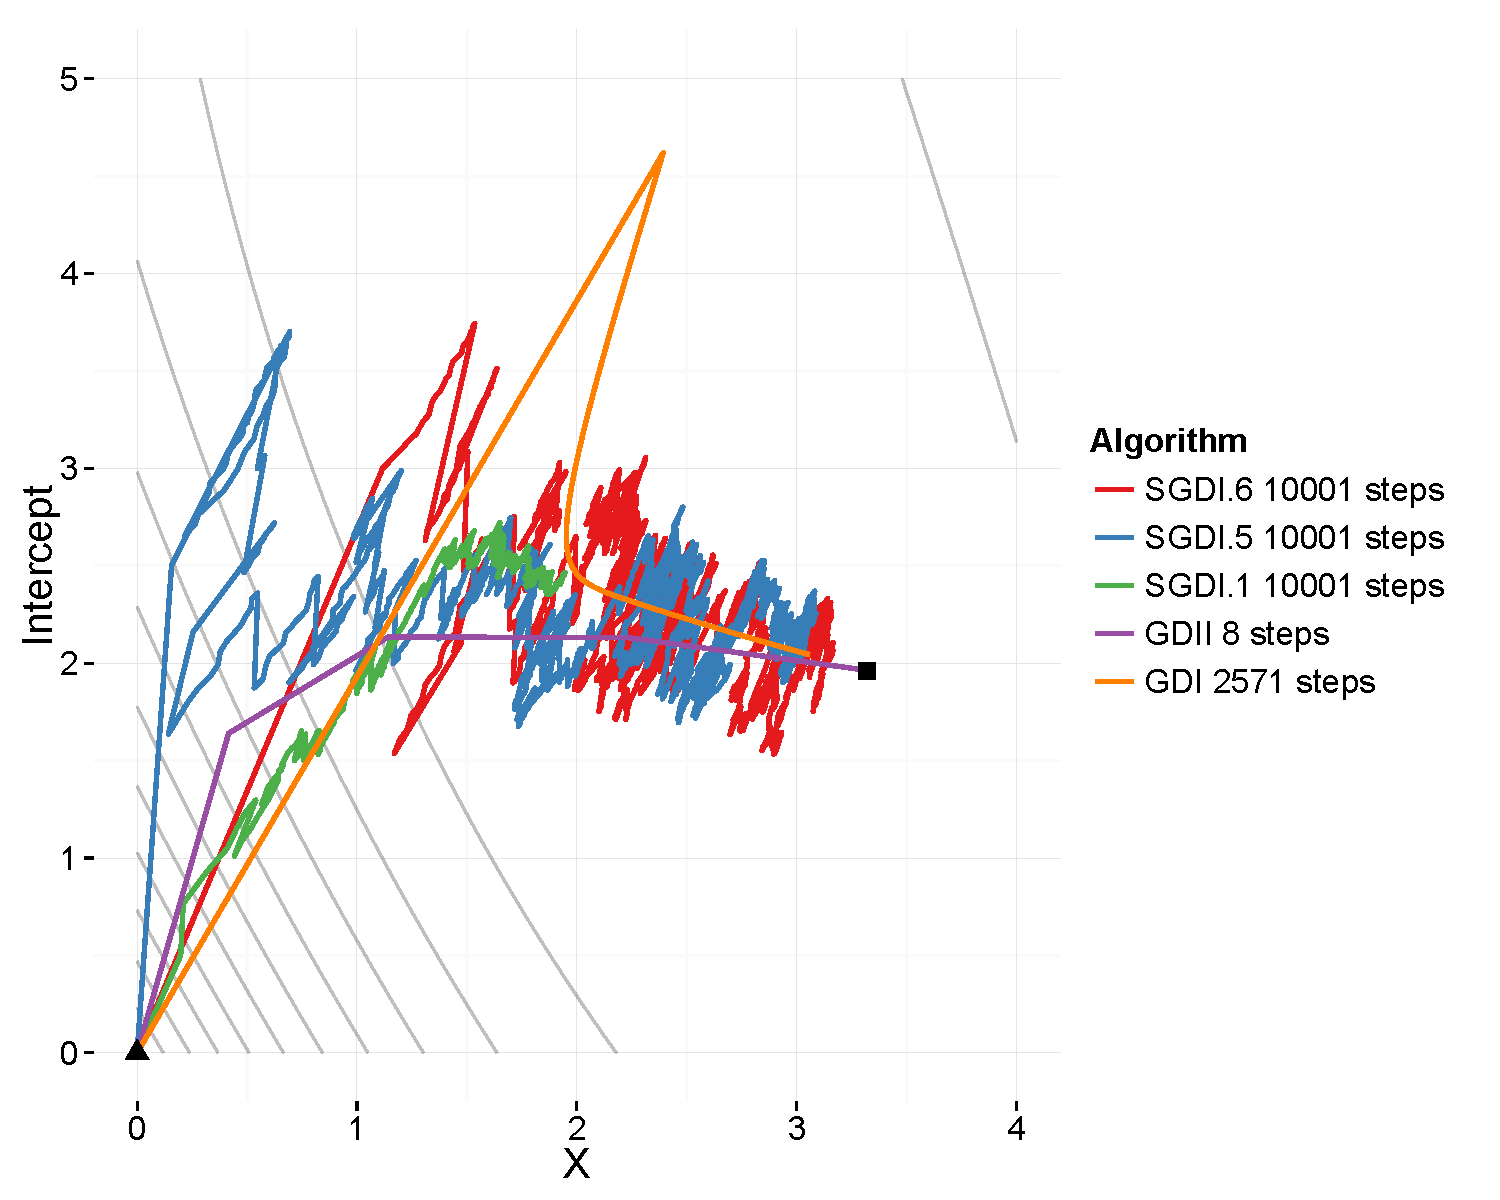
\includegraphics[width=\textwidth]{Obrazki/contour_00.pdf}
     \caption{Symulacja dla $\beta_0 = (0,0)$.}
   \end{subfigure}
   \begin{subfigure}[h!]{0.45\textwidth}
   %     \centering
        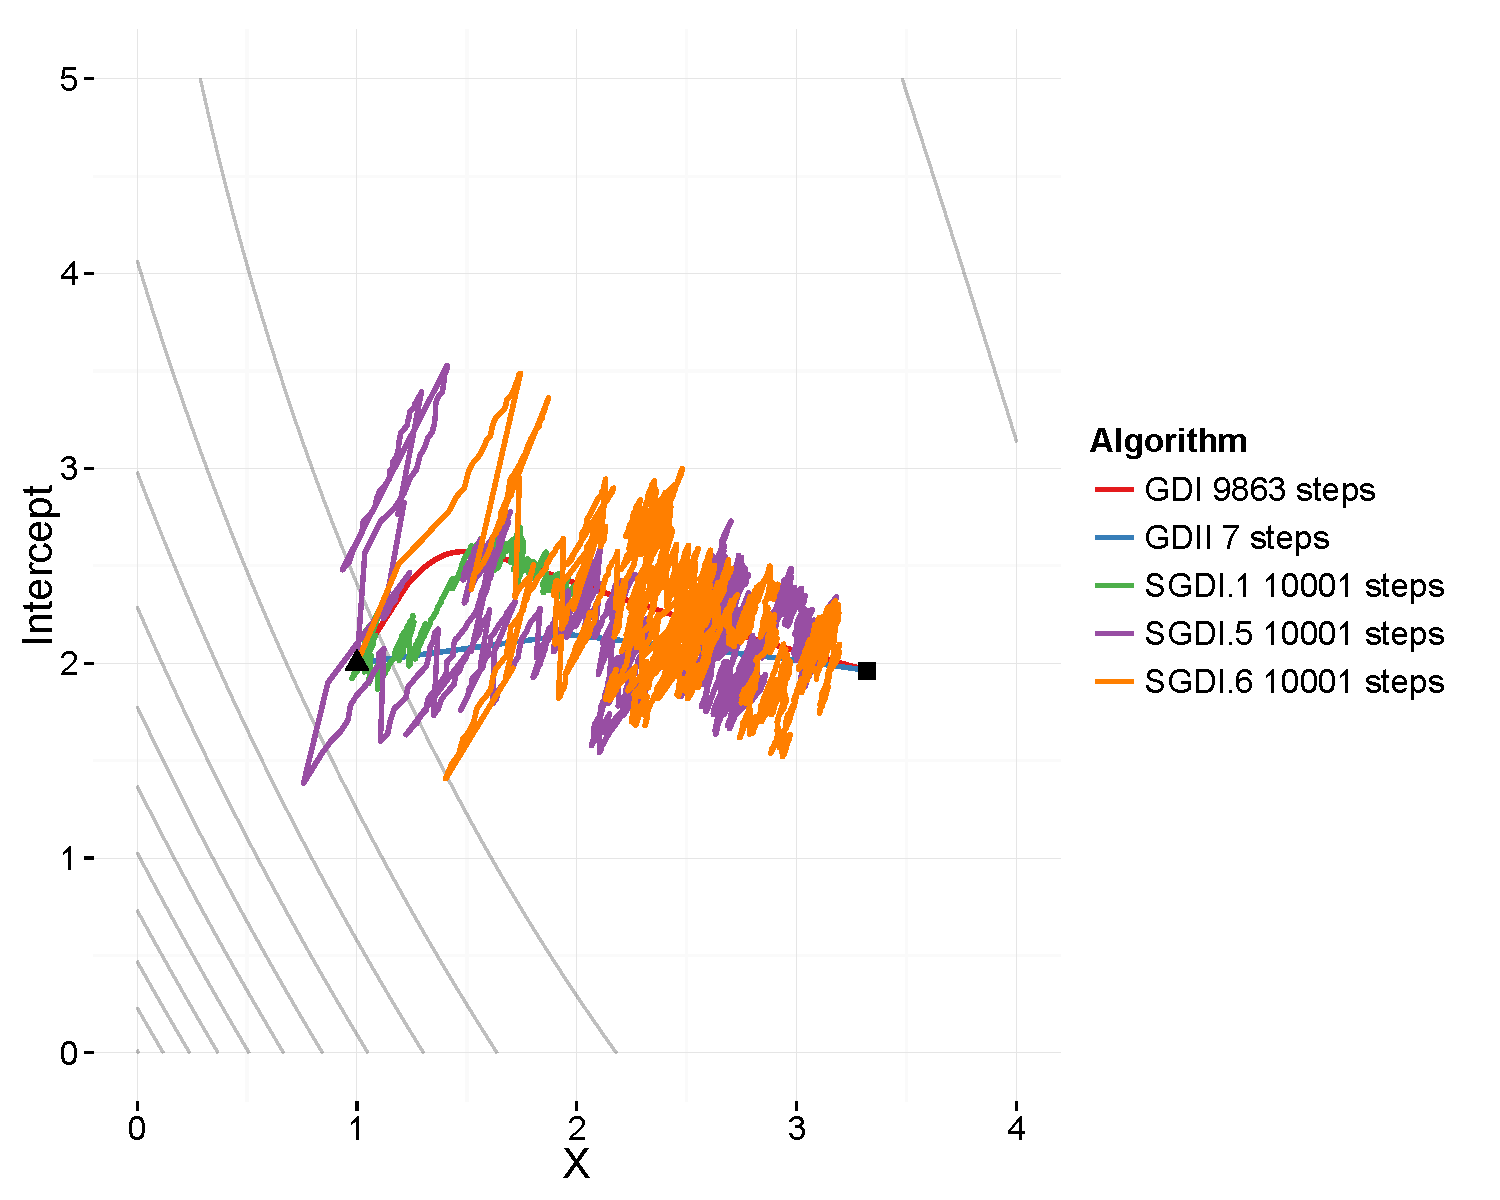
\includegraphics[width=\textwidth]{Obrazki/contour_2_1.pdf}
        \caption{Symulacja dla $\beta_0 = (1,2)$.}
      \end{subfigure}
   \begin{subfigure}[h!]{0.45\textwidth}
      %     \centering
           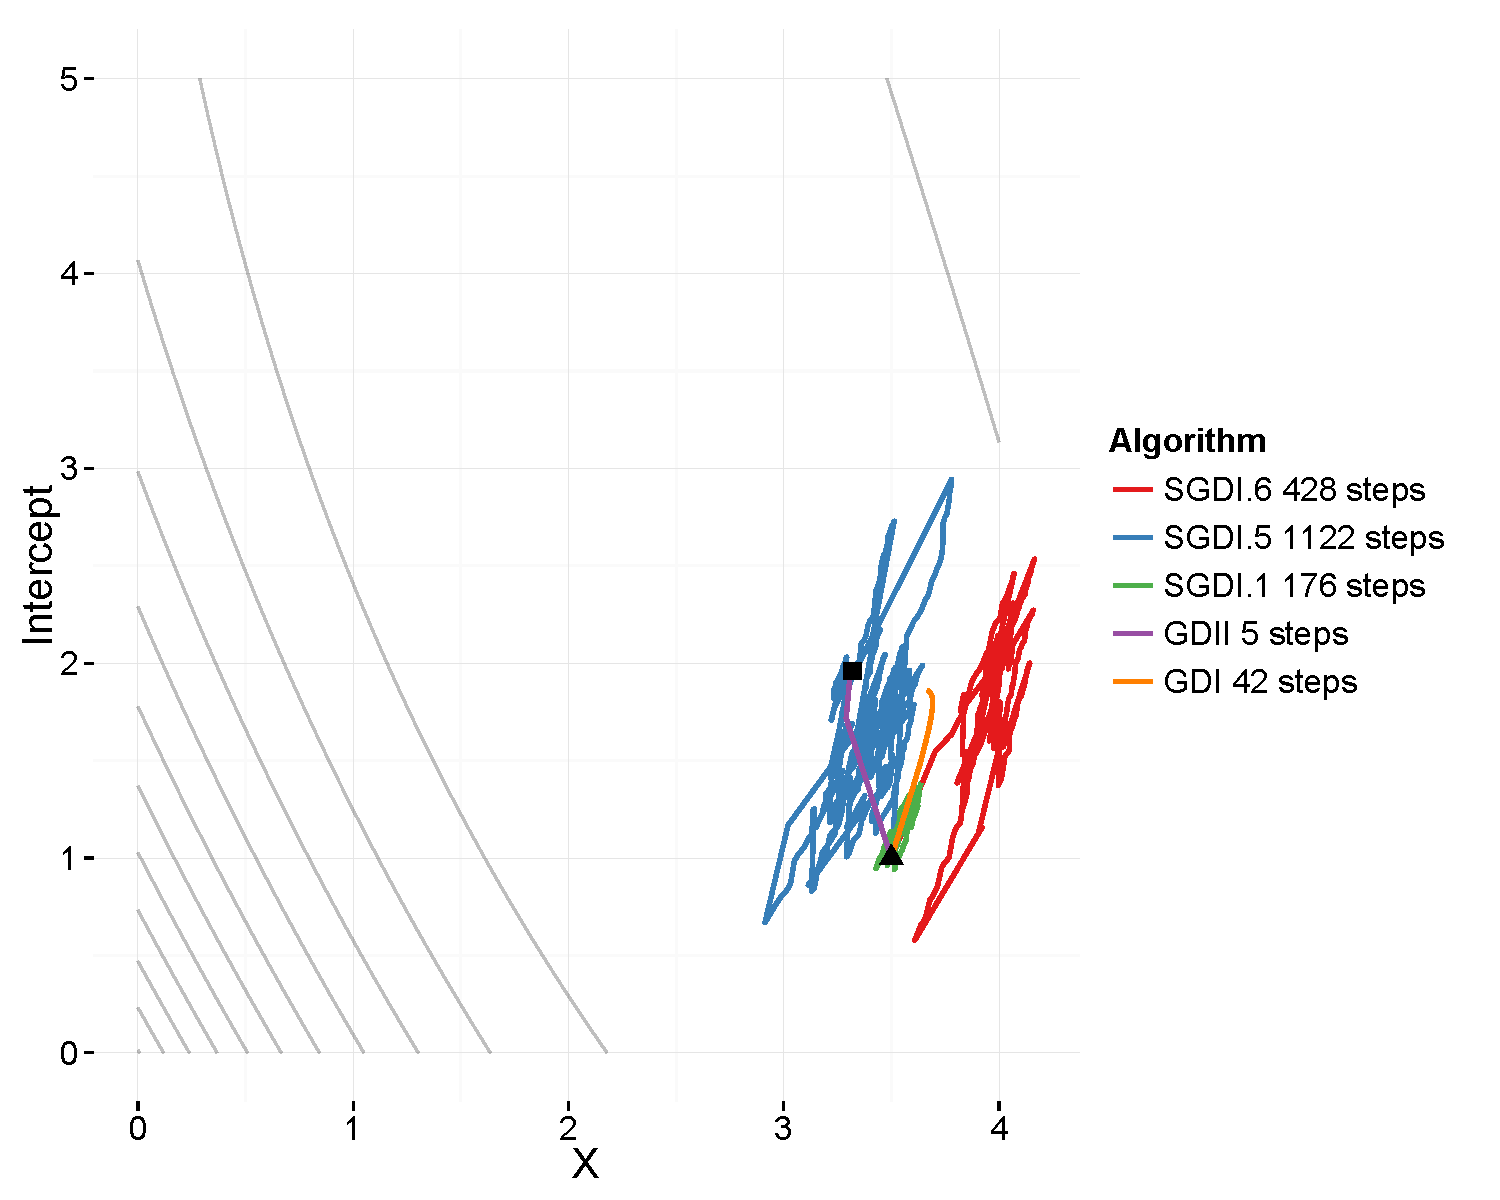
\includegraphics[width=\textwidth]{Obrazki/contour_35_1.pdf}
           \caption{Symulacja dla $\beta_0 = (3.5,1)$.}
                 \end{subfigure}
   \begin{subfigure}[h!]{0.45\textwidth}
         %     \centering
              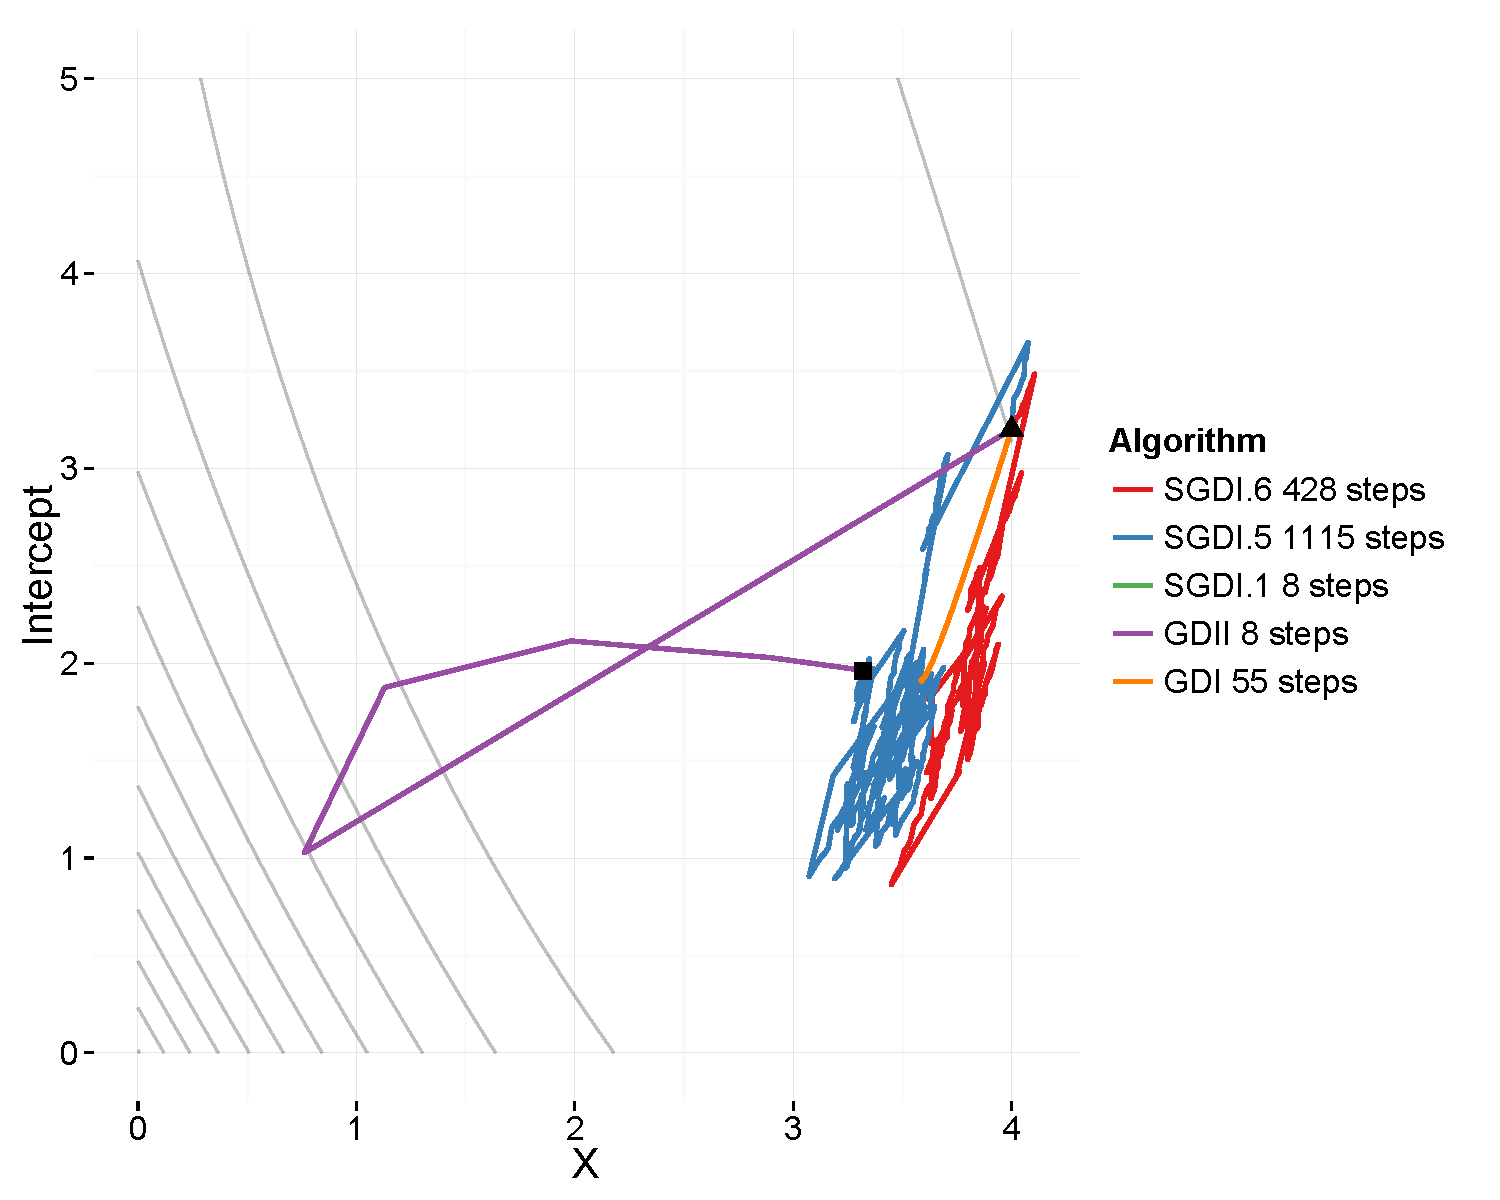
\includegraphics[width=\textwidth]{Obrazki/contour_4_32.pdf}
              \caption{Symulacja dla $\beta_0 = (4,3.2)$.}
            \end{subfigure}
\end{center}
\caption[Porównanie algorytmów spadku gradientu o wspólnym zakresie osi.]{\label{fig:sc5asd} Wykresy o wspólnym zakresie osi z zaznaczeniem warstwic funkcji log-wiarogodności dla modelu regresji logistycznej (równanie (\ref{logglm})). Wykresy przedstawiają porównanie algorytmów spadku gradientu. Początkowe dane losowano z innego ziarna losowania ustalone na 4561. Wykresy przedstawiają ścieżki zbieżności w kolejnych krokach algorytmów spadku gradientu. Ustalono maksymalną liczbę iteracji na 10001, zaś warunek stopu ustalono na $\varepsilon=10^{-4}$ ($\varepsilon=10^{-5}$ dla punktu startowego $\beta_0 = (0,0)$). Trójkątem zaznaczono punkt startowy, a kwadratem wyestymowane rozwiązanie przy pomocy funkcji \texttt{glm} \cite{glmglm}. Przez \texttt{GDI} oznaczono trajektoria dla algorytmu spadku gradientu rzędu I, przez \texttt{GDII} oznaczono trajektoria dla algorytmu spadku gradientu rzędu II, zaś przez \texttt{SGD.i} oznaczono 3 różne trajektorie dla algorytmów stochastycznego spadku gradientu dla różnych ciągów odpowiadających długości kroku algorytmu. Indeks $i$ odpowiada ciągowi wybranemu do wyznaczania długości kroku algorytmu na zasadzie $\alpha_{ki} = i/\sqrt{k}$.}
\end{figure}

Na kolejnych wykresach na Rysunkach \ref{fig:scasd} - \ref{fig:sc4asd} osie dopasowane są do obecnej symulacji. Ze względu na pomniejszenie zakresu osi, nie zdecydowano się na ukazanie warstwic.

\newpage

\begin{figure}[hbt!]
  %\vspace{-10pt}
  \begin{center}
   \begin{subfigure}[h!]{0.9\textwidth}
      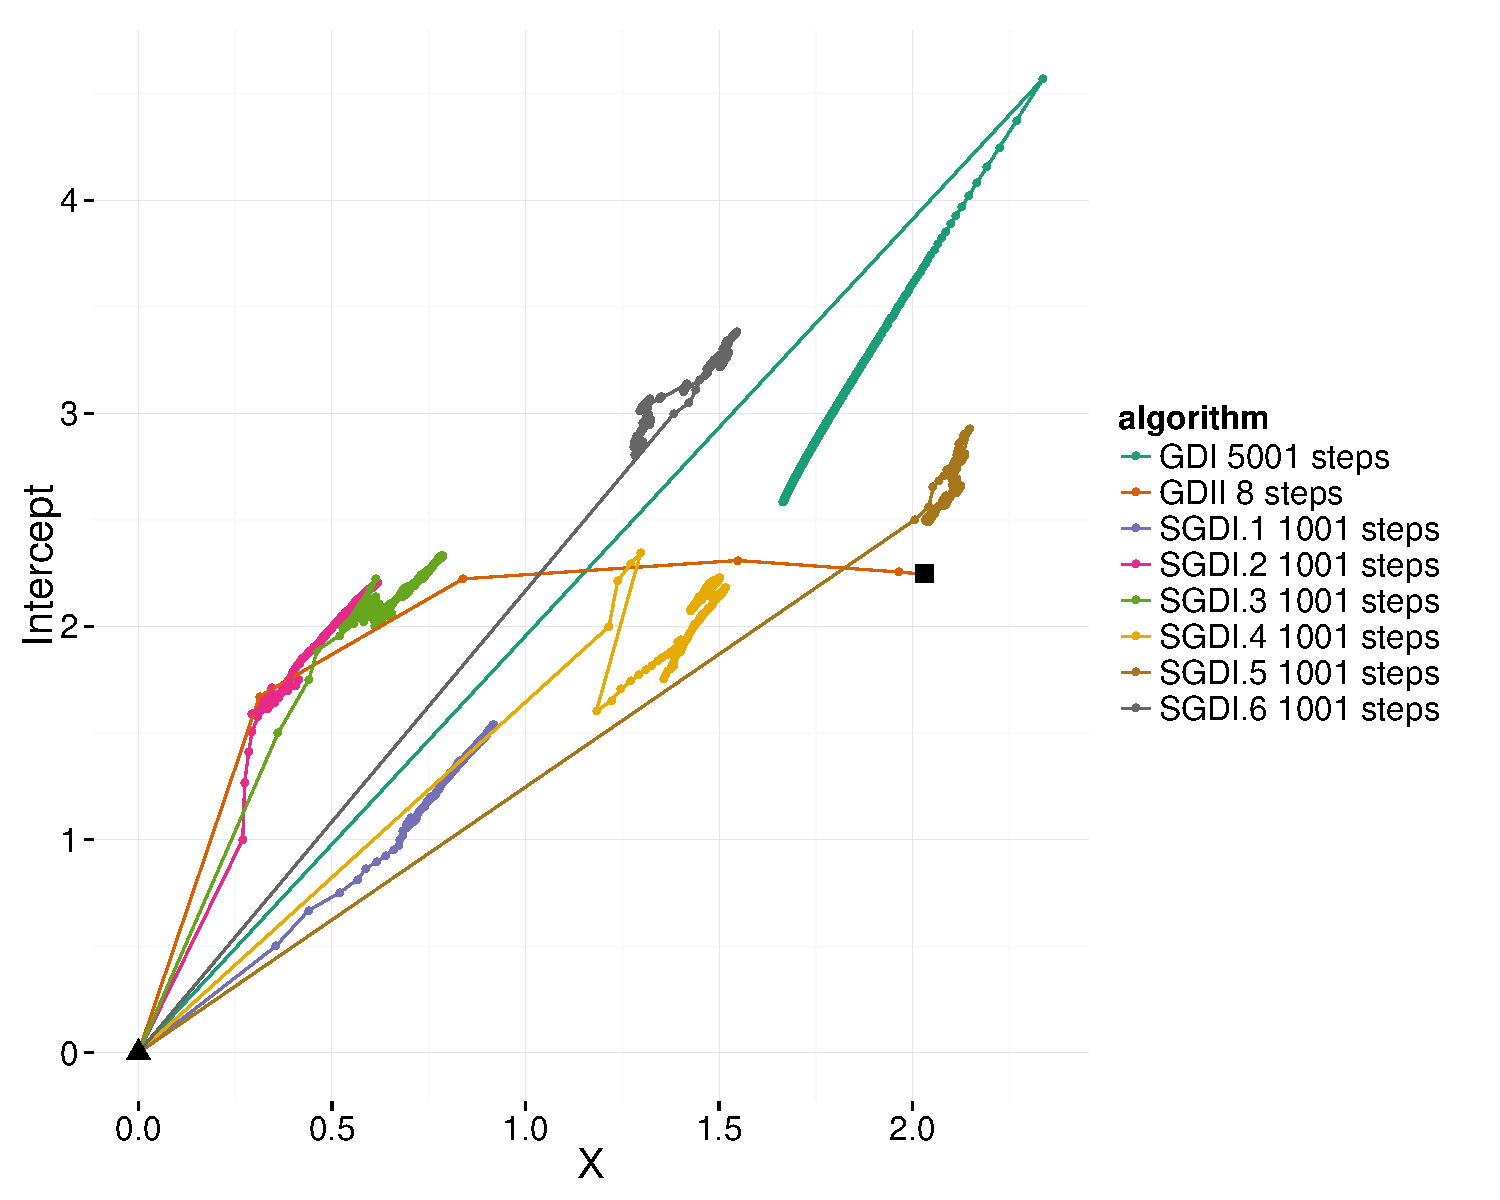
\includegraphics[width=\textwidth, height=270pt]{Obrazki/sgd_00_1.pdf}
      \caption{Symulacja dla $\beta_0 = (0,0)$ nr 1 dla ziarna losowania ustalonego na 4561.}
   \end{subfigure}     
   \begin{subfigure}[h!]{0.9\textwidth}
      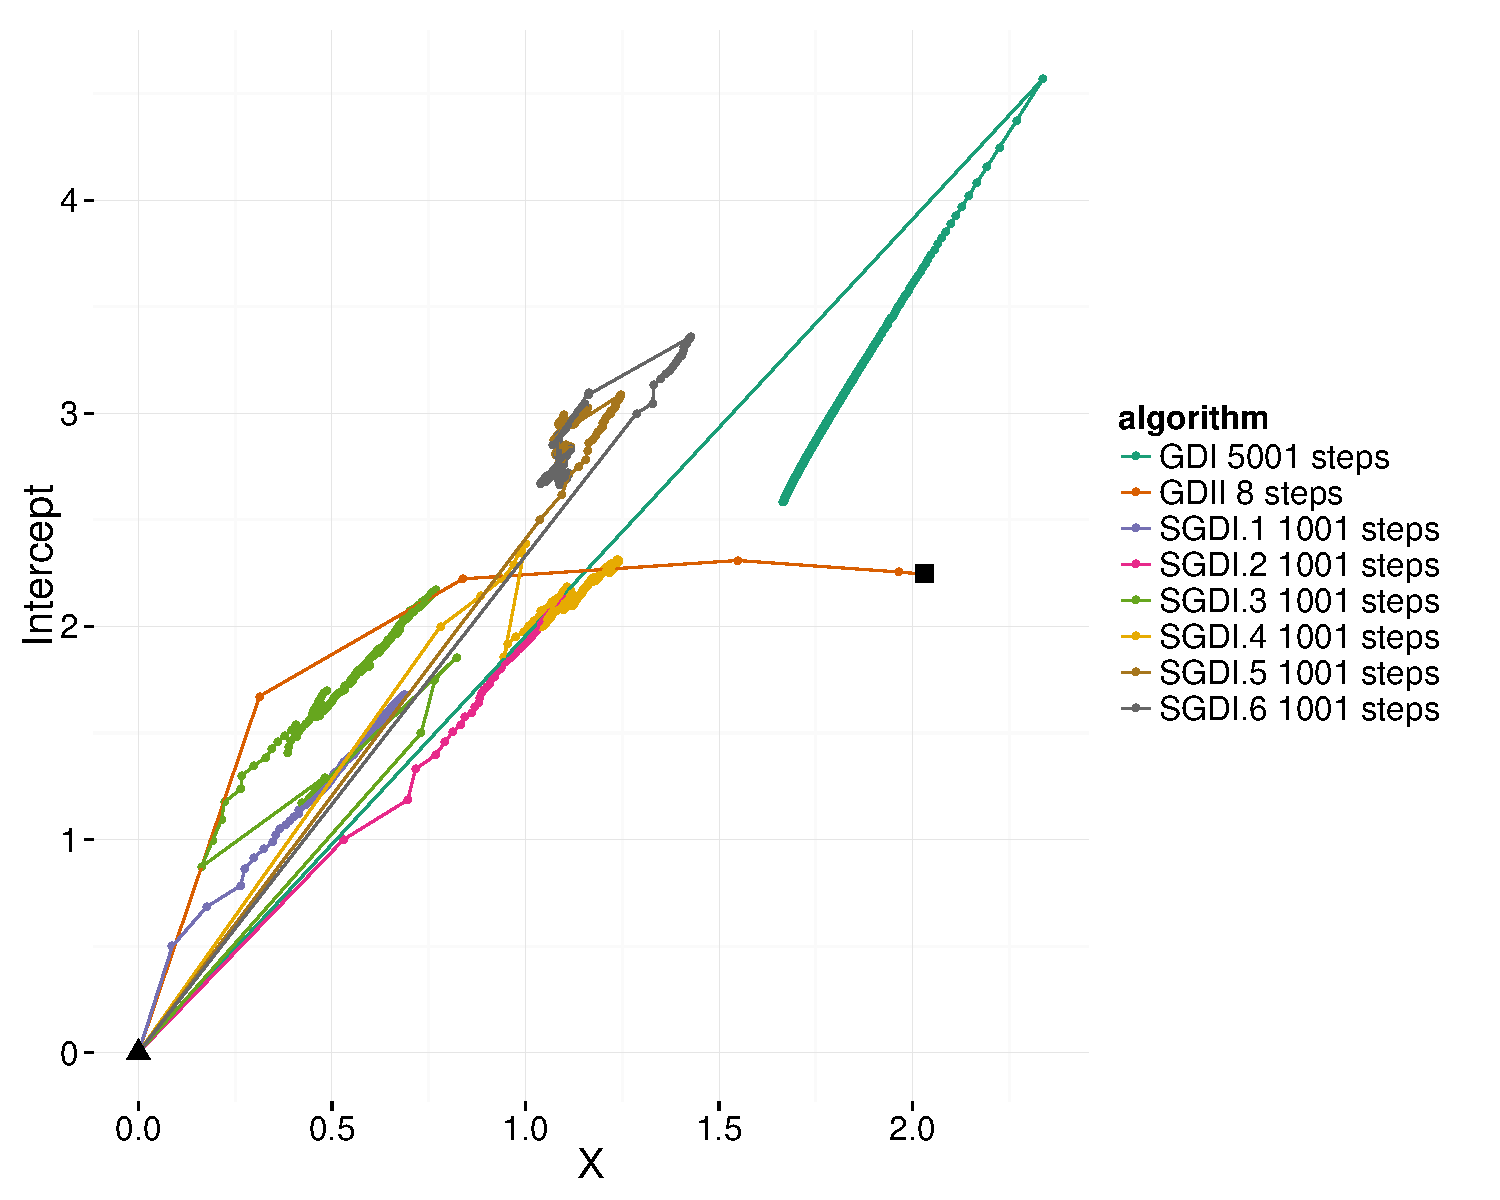
\includegraphics[width=\textwidth, height=270pt]{Obrazki/sgd_00_2.pdf}
      \caption{Symulacja dla $\beta_0 = (0,0)$ nr 2 dla ziarna losowania ustalonego na 456.}
   \end{subfigure}  \end{center}
  %\vspace{-10pt}
  \caption[Porównanie algorytmów spadku gradientu dla punktu startowego $\beta_0 = (0,0)$.]{\label{fig:scasd}Porównanie algorytmów spadku gradientu dla punktu startowego $\beta_0 = (0,0)$. Wykresy przedstawiają ścieżki zbieżności w kolejnych krokach algorytmów spadku gradientu. Ustalono maksymalną liczbę iteracji na 10001, zaś warunek stopu ustalono na $\varepsilon=10^{-5}$. Trójkątem zaznaczono punkt startowy, a kwadratem wyestymowane rozwiązanie przy pomocy funkcji \texttt{glm} \cite{glmglm}. Przez \texttt{GDI} oznaczono trajektoria dla algorytmu spadku gradientu rzędu I, przez \texttt{GDII} oznaczono trajektoria dla algorytmu spadku gradientu rzędu II, zaś przez \texttt{SGD.i} oznaczono 3 różne trajektorie dla algorytmów stochastycznego spadku gradientu dla różnych ciągów odpowiadających długości kroku algorytmu. Indeks $i$ odpowiada ciągowi wybranemu do wyznaczania długości kroku algorytmu na zasadzie $\alpha_{ki} = i/\sqrt{k}$.}
\end{figure}


\begin{figure}[hbt!]
  %\vspace{-10pt}
  \begin{center}
   \begin{subfigure}[h!]{0.9\textwidth}
      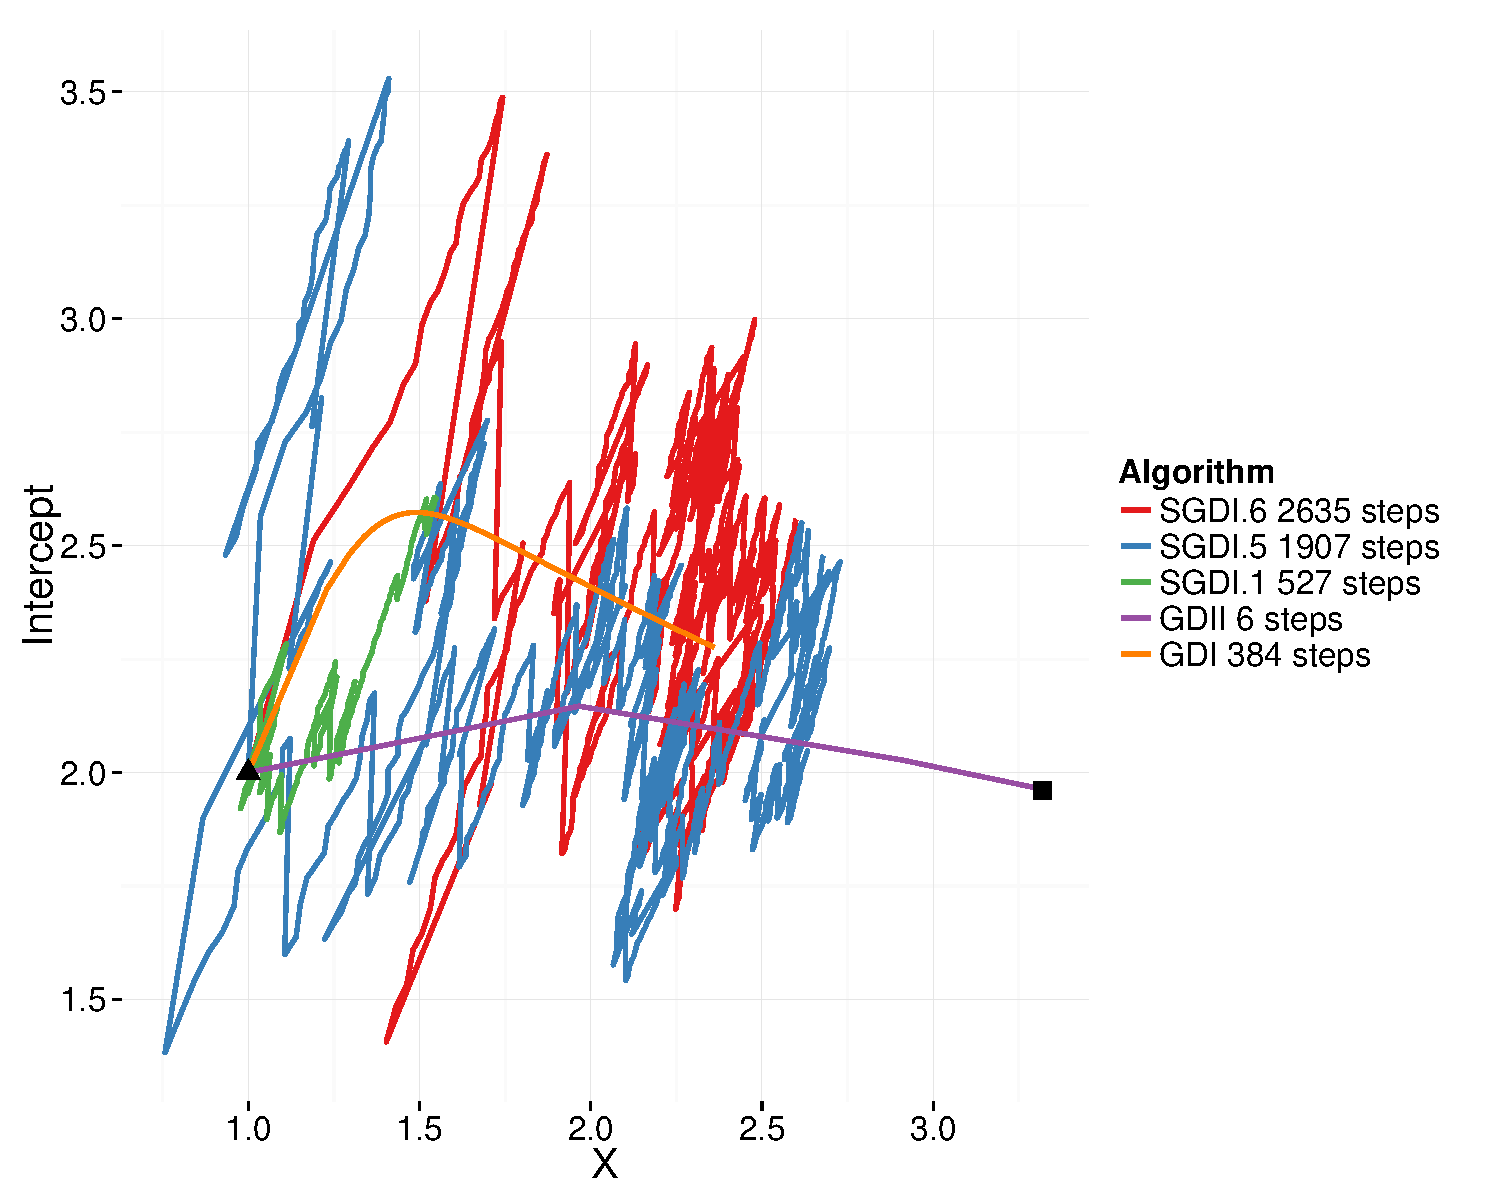
\includegraphics[width=\textwidth, height=270pt]{Obrazki/sgd_1_2_1.pdf}
      \caption{Symulacja dla $\beta_0 = (1,2)$ nr 1 dla ziarna losowania ustalonego na 4561.}
   \end{subfigure}     
   \begin{subfigure}[h!]{0.9\textwidth}
      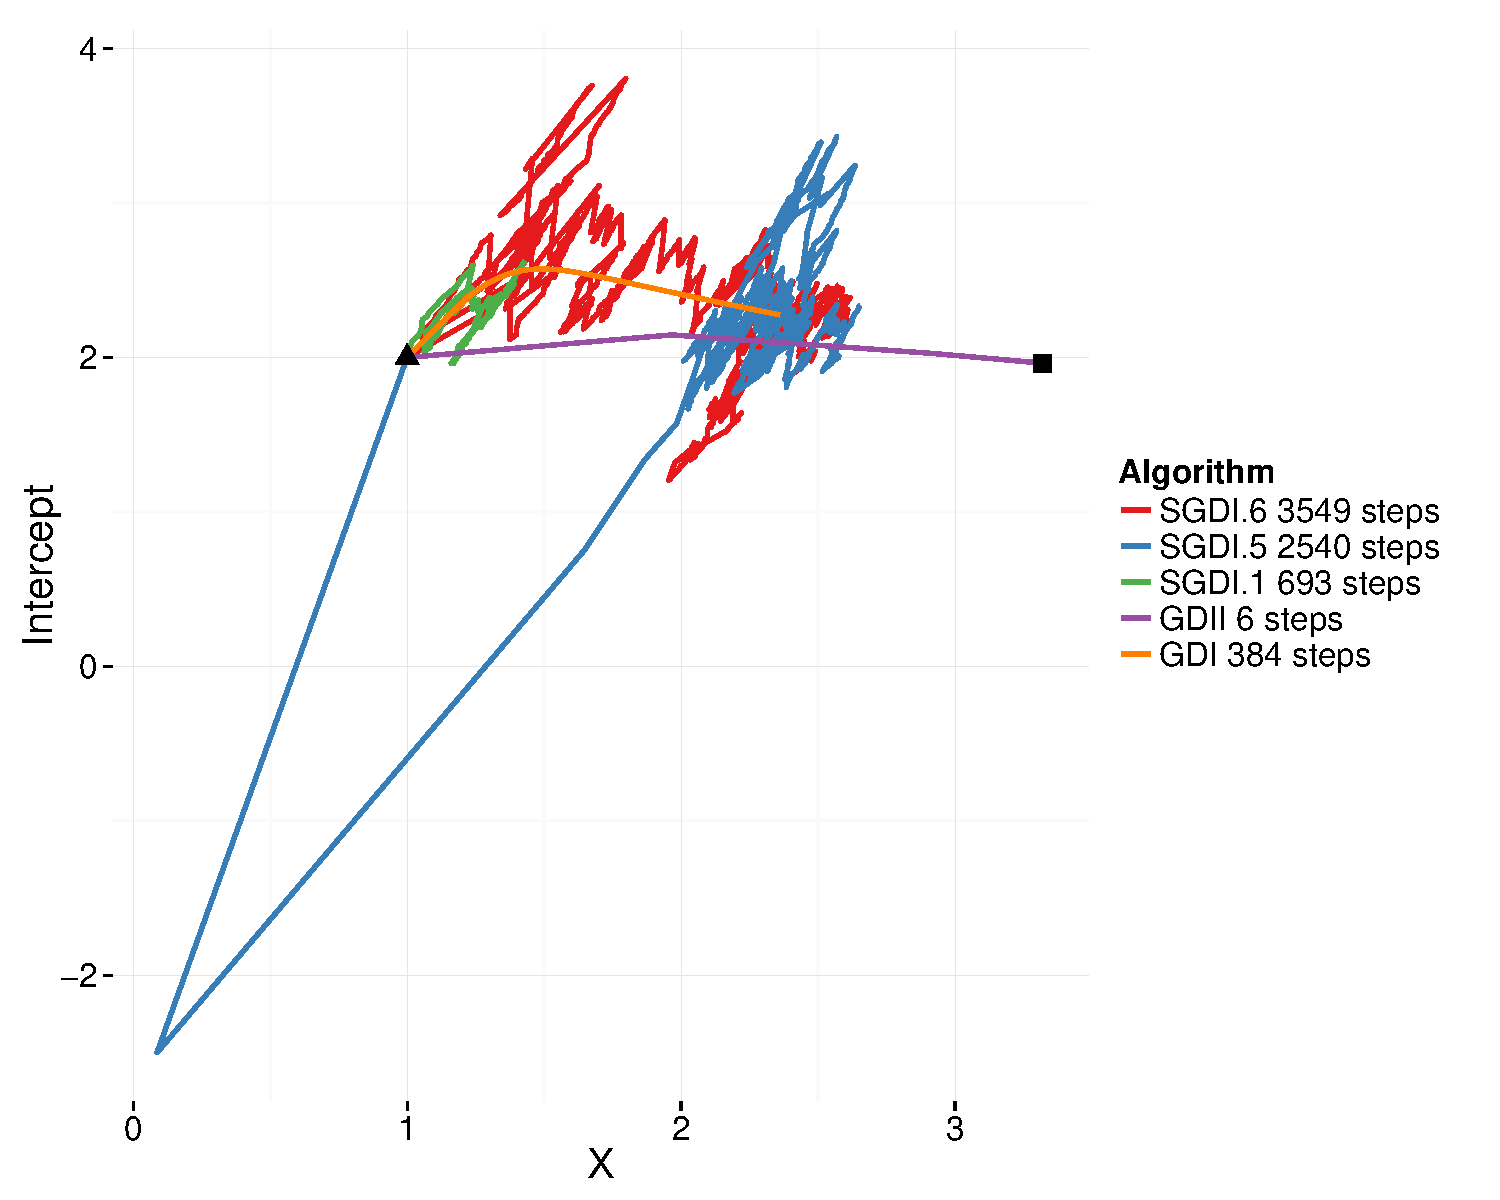
\includegraphics[width=\textwidth, height=270pt]{Obrazki/sgd_1_2_2.pdf}
      \caption{Symulacja dla $\beta_0 = (1,2)$ nr 2 dla ziarna losowania ustalonego na 456.}
   \end{subfigure}  \end{center}
  %\vspace{-10pt}
  \caption[Porównanie algorytmów spadku gradientu dla punktu startowego $\beta_0 = (1,2)$.]{\label{fig:sc2asd}Porównanie algorytmów spadku gradientu dla punktu startowego $\beta_0 = (1,2)$. Wykresy przedstawiają ścieżki zbieżności w kolejnych krokach algorytmów spadku gradientu. Ustalono maksymalną liczbę iteracji na 10001, zaś warunek stopu ustalono na $\varepsilon=10^{-4}$. Trójkątem zaznaczono punkt startowy, a kwadratem wyestymowane rozwiązanie przy pomocy funkcji \texttt{glm} \cite{glmglm}. Przez \texttt{GDI} oznaczono trajektoria dla algorytmu spadku gradientu rzędu I, przez \texttt{GDII} oznaczono trajektoria dla algorytmu spadku gradientu rzędu II, zaś przez \texttt{SGD.i} oznaczono 3 różne trajektorie dla algorytmów stochastycznego spadku gradientu dla różnych ciągów odpowiadających długości kroku algorytmu. Indeks $i$ odpowiada ciągowi wybranemu do wyznaczania długości kroku algorytmu na zasadzie $\alpha_{ki} = i/\sqrt{k}$.}
\end{figure}


\begin{figure}[hbt!]
  %\vspace{-10pt}
  \begin{center}
   \begin{subfigure}[h!]{0.9\textwidth}
      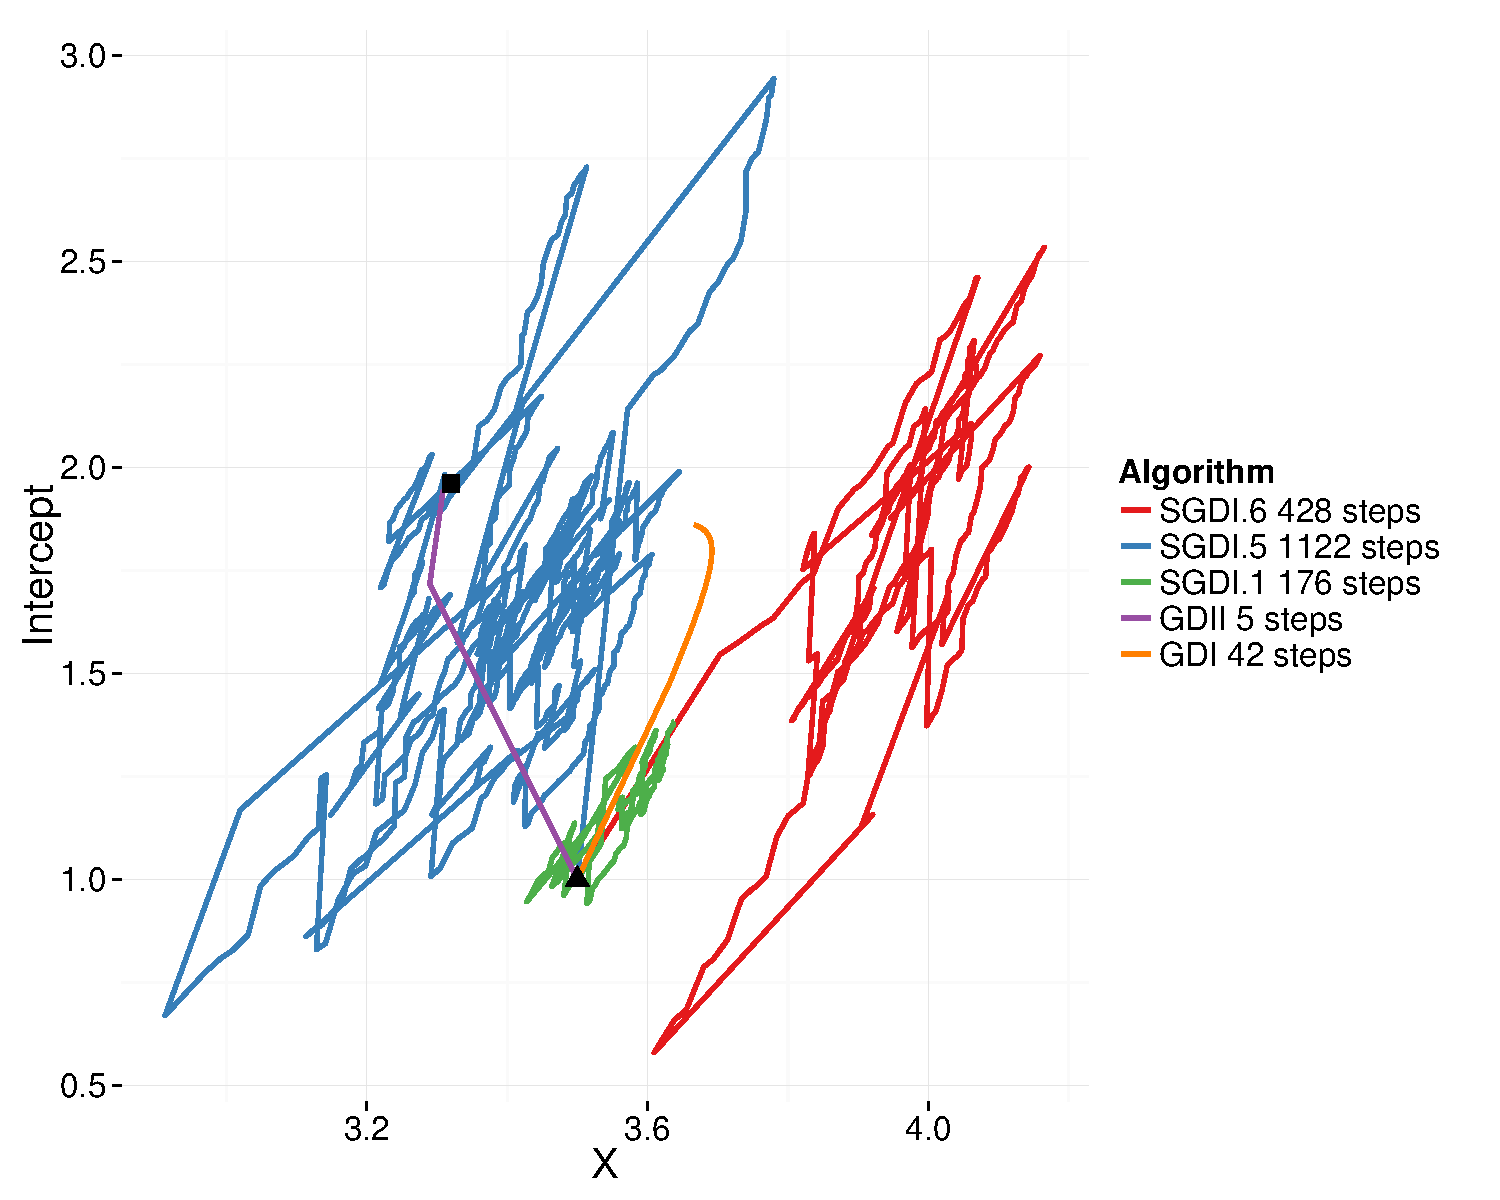
\includegraphics[width=\textwidth, height=270pt]{Obrazki/sgd_35_1_1.pdf}
      \caption{Symulacja dla $\beta_0 = (3.5,1)$ nr 1 dla ziarna losowania ustalonego na 4561.}
   \end{subfigure}     
   \begin{subfigure}[h!]{0.9\textwidth}
      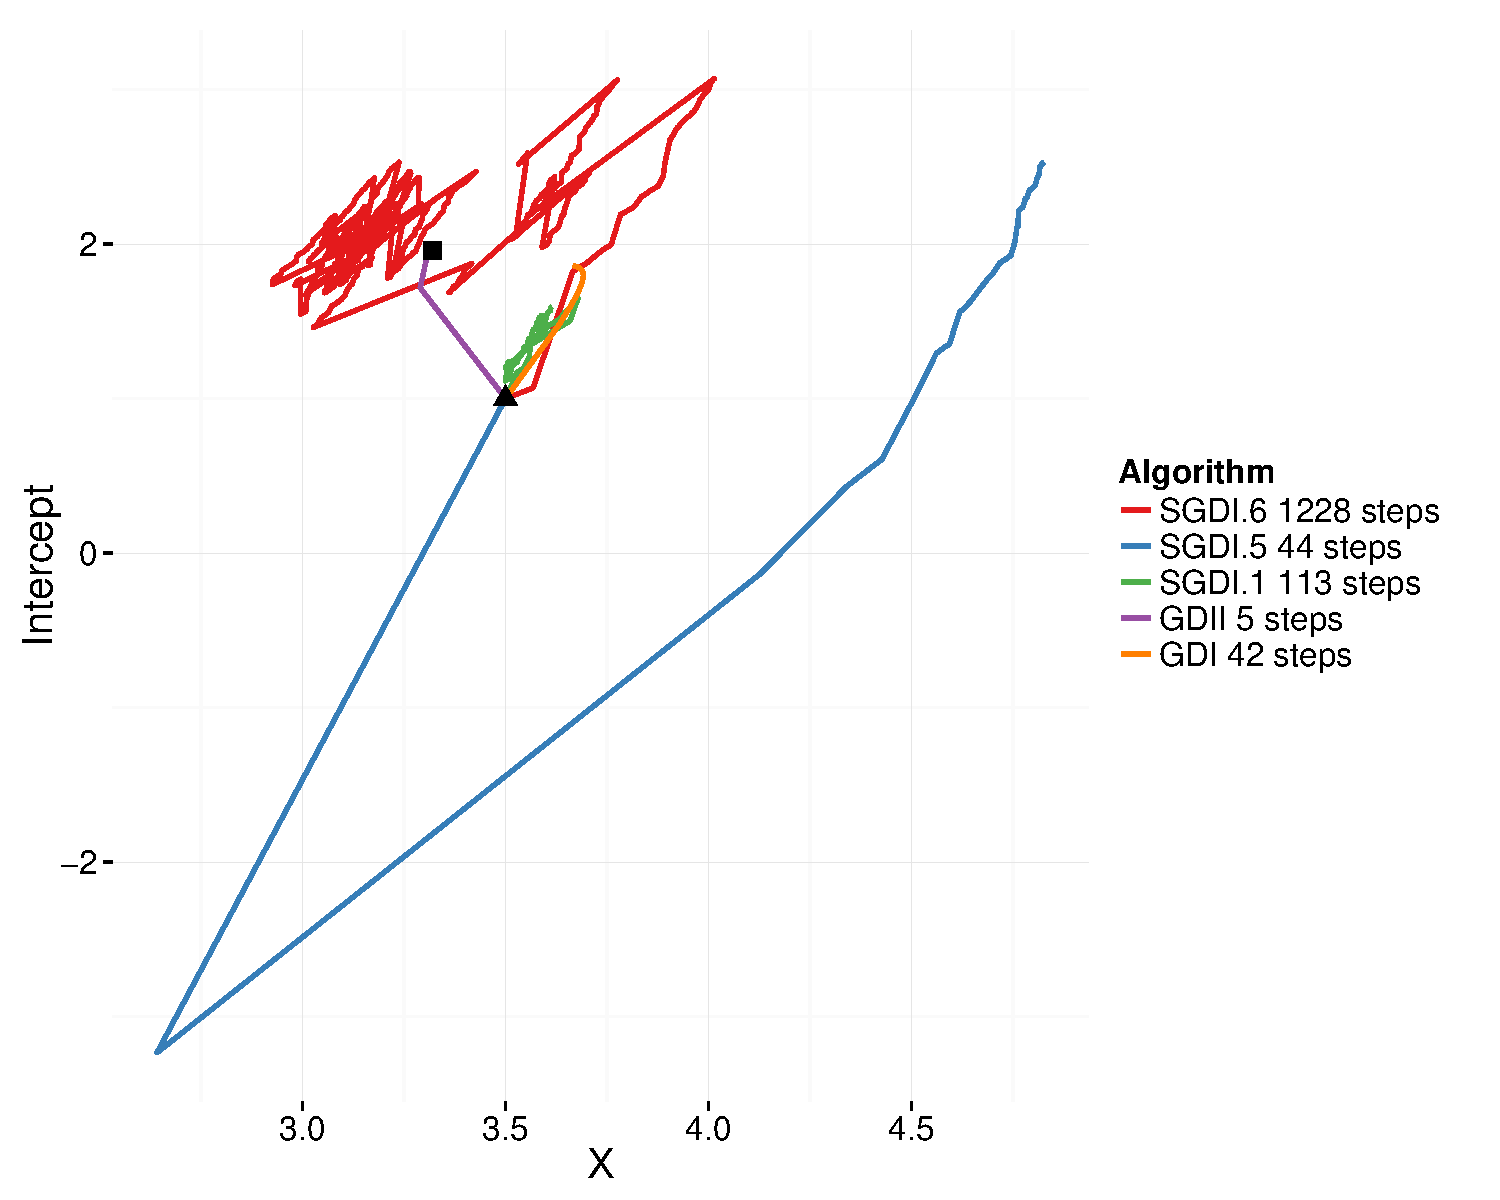
\includegraphics[width=\textwidth, height=270pt]{Obrazki/sgd_35_1_2.pdf}
      \caption{Symulacja dla $\beta_0 = (3.5,1)$ nr 2 dla ziarna losowania ustalonego na 456.}
   \end{subfigure}  \end{center}
  %\vspace{-10pt}
  \caption[Porównanie algorytmów spadku gradientu dla punktu startowego $\beta_0 = (3.5,1)$.]{\label{fig:sc3asd}Porównanie algorytmów spadku gradientu dla punktu startowego $\beta_0 = (3.5,1)$. Wykresy przedstawiają ścieżki zbieżności w kolejnych krokach algorytmów spadku gradientu. Ustalono maksymalną liczbę iteracji na 10001, zaś warunek stopu ustalono na $\varepsilon=10^{-4}$. Trójkątem zaznaczono punkt startowy, a kwadratem wyestymowane rozwiązanie przy pomocy funkcji \texttt{glm} \cite{glmglm}. Przez \texttt{GDI} oznaczono trajektoria dla algorytmu spadku gradientu rzędu I, przez \texttt{GDII} oznaczono trajektoria dla algorytmu spadku gradientu rzędu II, zaś przez \texttt{SGD.i} oznaczono 3 różne trajektorie dla algorytmów stochastycznego spadku gradientu dla różnych ciągów odpowiadających długości kroku algorytmu. Indeks $i$ odpowiada ciągowi wybranemu do wyznaczania długości kroku algorytmu na zasadzie $\alpha_{ki} = i/\sqrt{k}$.}
\end{figure}


\begin{figure}[hbt!]
  %\vspace{-10pt}
  \begin{center}
   \begin{subfigure}[h!]{0.9\textwidth}
      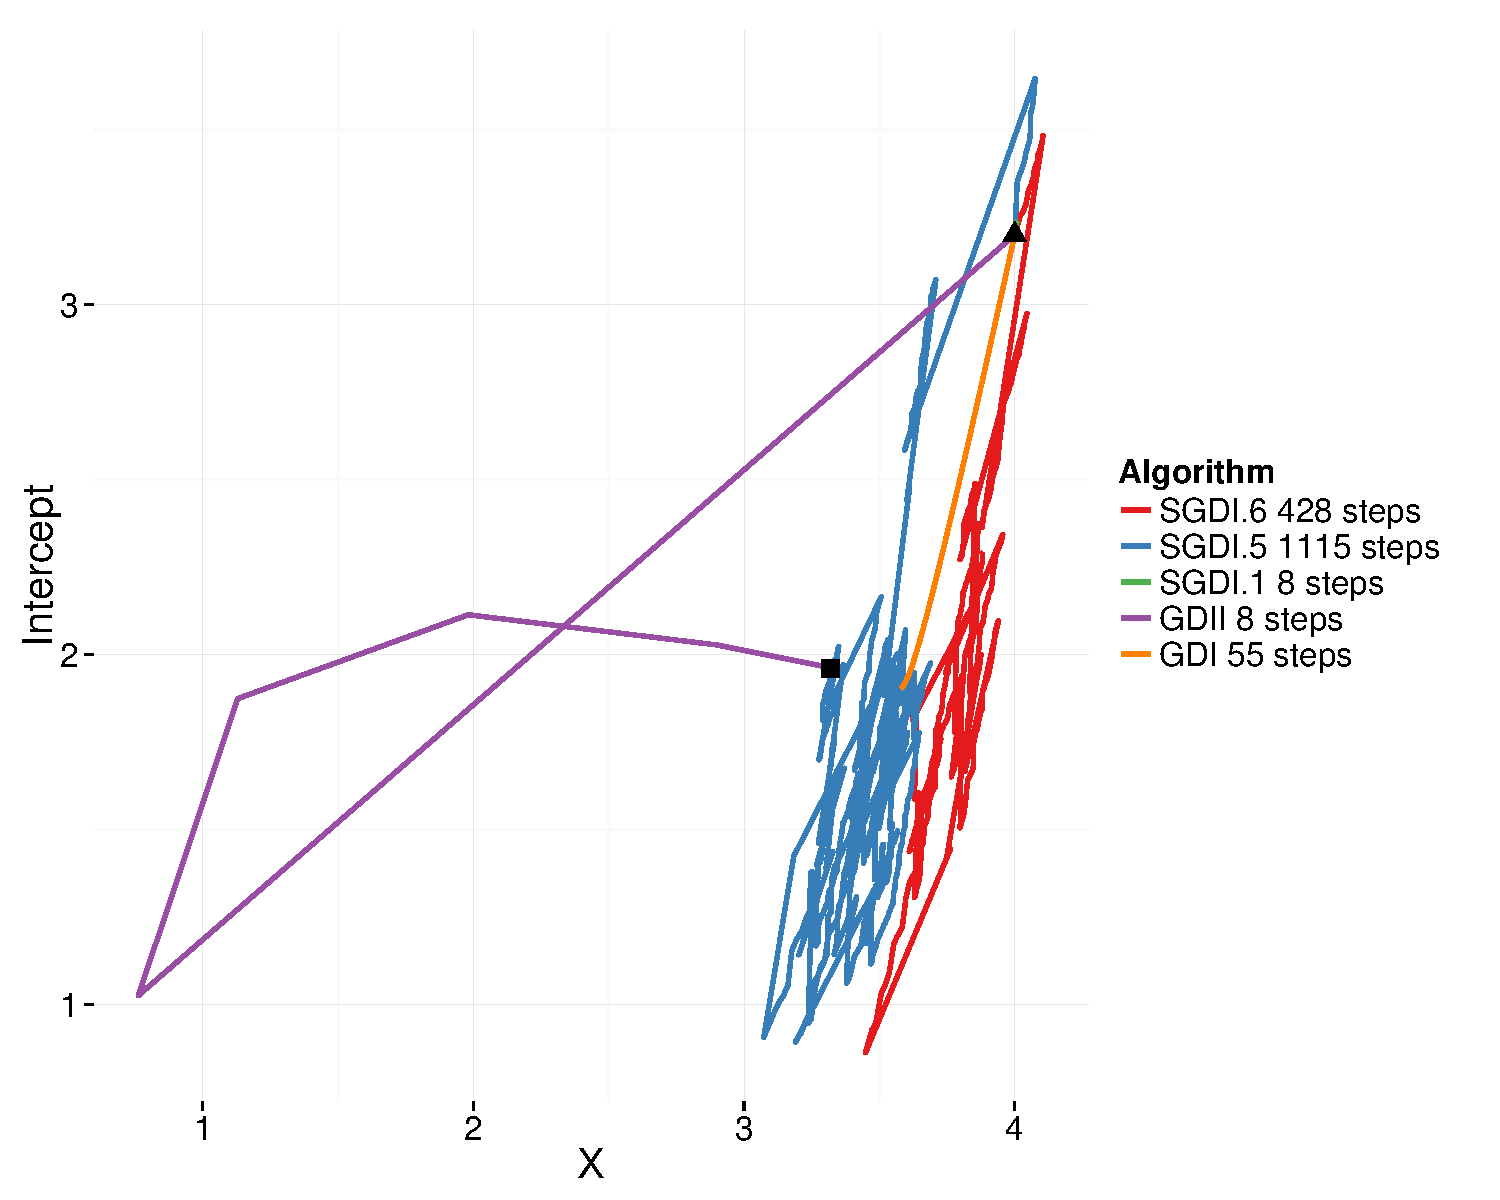
\includegraphics[width=\textwidth, height=270pt]{Obrazki/sgd_32_4_1.pdf}
      \caption{Symulacja dla $\beta_0 = (4,3.2)$ nr 1 dla ziarna losowania ustalonego na 4561.}
   \end{subfigure}     
   \begin{subfigure}[h!]{0.9\textwidth}
      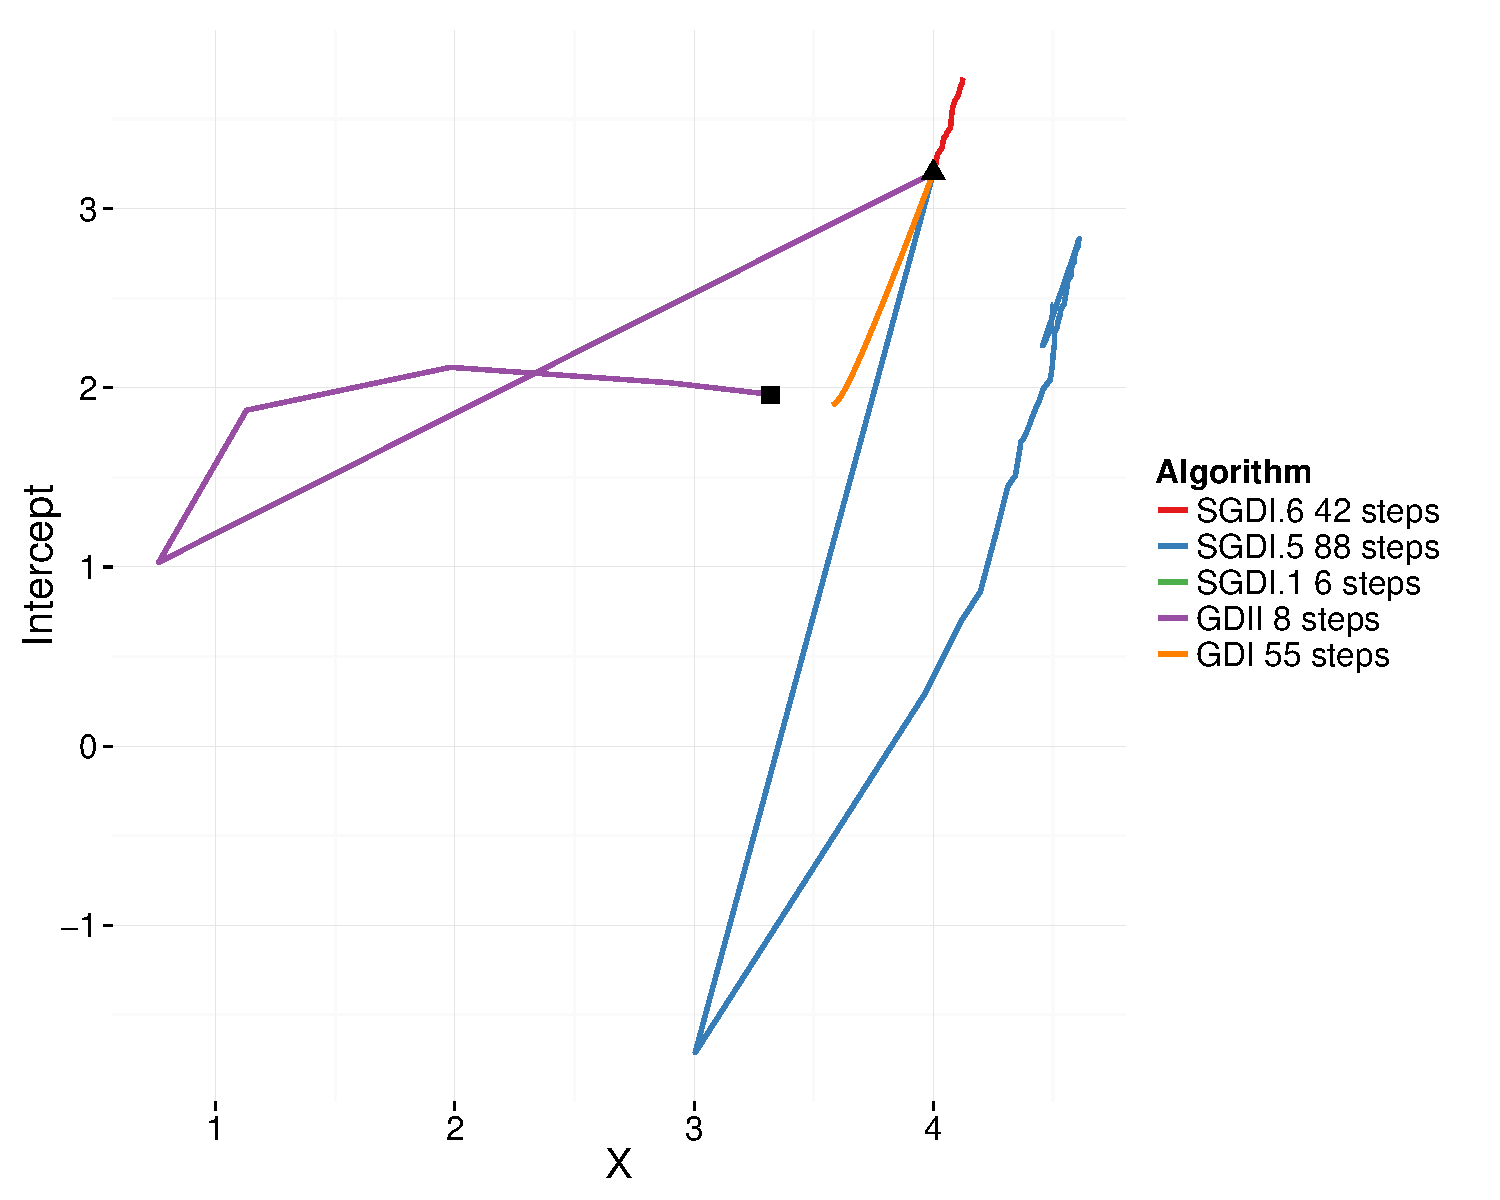
\includegraphics[width=\textwidth, height=270pt]{Obrazki/sgd_32_4_2.pdf}
      \caption{Symulacja dla $\beta_0 = (4,3.2)$ nr 2 dla ziarna losowania ustalonego na 456.}
   \end{subfigure}  \end{center}
  %\vspace{-10pt}
  \caption[Porównanie algorytmów spadku gradientu dla punktu startowego $\beta_0 = (4,3.2)$.]{\label{fig:sc4asd}Porównanie algorytmów spadku gradientu dla punktu startowego $\beta_0 = (4,3.2)$. Wykresy przedstawiają ścieżki zbieżności w kolejnych krokach algorytmów spadku gradientu. Ustalono maksymalną liczbę iteracji na 10001, zaś warunek stopu ustalono na $\varepsilon=10^{-4}$. Trójkątem zaznaczono punkt startowy, a kwadratem wyestymowane rozwiązanie przy pomocy funkcji \texttt{glm} \cite{glmglm}. Przez \texttt{GDI} oznaczono trajektoria dla algorytmu spadku gradientu rzędu I, przez \texttt{GDII} oznaczono trajektoria dla algorytmu spadku gradientu rzędu II, zaś przez \texttt{SGD.i} oznaczono 3 różne trajektorie dla algorytmów stochastycznego spadku gradientu dla różnych ciągów odpowiadających długości kroku algorytmu. Indeks $i$ odpowiada ciągowi wybranemu do wyznaczania długości kroku algorytmu na zasadzie $\alpha_{ki} = i/\sqrt{k}$.}
\end{figure}


\newpage

\subsubsection{Podsumowanie symulacji}
W trackie symulacji badano zachowanie trajektorii zbieżności w kolejnych krokach algorytmów spadku gradientu. Algorytm spadku gradientu rzędu II zbiegał do rozwiązania wyznaczonego przez funkcję \texttt{glm} \cite{glmglm} i osiągał zbieżność po najmniejszej liczbie kroków, jednak należy pamiętać o kosztownych obliczeniowo operacjach odwracania macierzy Hesjanu wykonywanych w trakcie optymalizacji z wykorzystaniem tej metody. 

Algorytm spadku gradientu rzędu I zbiegał do rozwiązania wyznaczonego przez funkcję \texttt{glm} w sytuacjach, gdy warunek stopu algorytmu był dostatecznie mały ($\varepsilon = 10^{-5}$, Rysunek \ref{fig:scasd}) oraz był na dobrej drodze do rozwiązania jednak nie dotarł do tych samych punktów co algorytm spadku gradientu rzędu II z racji na zbyt duży warunek stopu ($\varepsilon = 10^{-4}$, Rysunki \ref{fig:sc2asd} i \ref{fig:sc4asd}). Dla punktu startowego bliskiego rozwiązaniu pochodzącemu z wyliczeń z funkcji \texttt{glm} i dużego warunku stopu algorytmu algorytm spadku gradientu rzędu I miał problem z obraniem właściwego toru zbieżności do rozwiązania i ostatecznie wypadł najgorzej z wszystkich sprawdzanych algorytmów. Estymacja w tym wypadku dla algorytmu spadku gradientu rzędu I miała najmniej kroków, co może wynikać z mało różnowartościowych wartości optymalizowanej funkcji log-wiarogodności w badanym obszarze będącym stosunkowo blisko rozwiązania znalezionego przez funkcję \texttt{glm}.

W przypadku stochastycznego spadku gradientu widać duże wahania w trajektoriach zbieżności algorytmu. W ramach symulacji badano wiele ciągów odpowiadających za długość kroku w tym algorytmie i ostatecznie zdecydowano ukazać w pracy ciągi, dla których osiągana była zbieżność dla największej liczby punktów startowych. Algorytm \texttt{SGDI.1} w każdym z możliwych przypadków miał zbyt małe wartości ciągu odpowiadającego za długości kroków algorytmu przez co nie dochodził do punktu wyliczonego przez funkcję \texttt{glm}, a ukazany został aby uświadomić jak ważnym aspektem jest odpowiednie dobranie długości kroków. Dla odpowiednio dobranego ciągu długości kroków o dużych wartościach jakim był ciąg $\alpha_{ki} = i/\sqrt{k}, i = 5, 6$ w wielu sytuacjach doszło do zbieżności w tym samym punkcie, w którym zbiegł algorytm zaimplementowany w funkcji \texttt{glm}. Najlepiej widać to na Rysunku \ref{fig:scasd} ($\varepsilon = 10^{-5}$) oraz Rysunku \ref{fig:sc2asd} ($\varepsilon = 10^{-4}$), gdzie w zbieżności algorytmu przeszkodził zbyt duży warunek stopu. Ciekawy rezultat osiągnięto na Rysunku \ref{fig:sc3asd}, gdzie dla różnych początkowych ziaren losowości osiągnięto zbieżność do punktu wyliczonego przez funkcję \texttt{glm} za każdym razem dla innego z dwóch poważnie rozważanych przypadków \texttt{SGDI.5}, \texttt{SGDI.6}. Istota losowości odgrywa kluczową rolę w algorytmie stochastycznego spadku gradientu i należy mieć świadomość, że dla różnych ziaren losowości, a co za tymi idzie dla innej kolejności obserwacji uwzględnianych w kolejnych krokach optymalizacji, algorytm może zachowywać się różnie. Doskonale widać to na Rysunku \ref{fig:sc4asd}, gdzie dla Symulacji nr 1 jeden przypadek algorytmu stochastycznego spadku gradientu osiągnął lepsze wyniki niż spadek gradientu rzędu I, zaś dla Symulacji nr 2 żadna wersja stochastyczna nie miała trajektorii zgodnych z prawdziwym kierunkiem zbieżności.

Ostatecznie można stwierdzić, że w wielu przypadkach stochastyczny wariant estymacji w przypadku optymalizacji funkcji log-wiarogodności dla modelu regresji logistycznej daje zadowalające rezultaty, które są niekiedy podobne do tych osiągniętych dzięki algorytmom spadku gradientu. Dzieje się to jednak po właściwym dobraniu ciągu odpowiadającego za długości poszczególnych kroków w algorytmie oraz po odpowiednim wyznaczeniu warunku stopu algorytmu. Należy pamiętać, że jest to jednak algorytm stochastyczny i istnieją nieliczne sytuacje, w których osiągnięte dzięki niemu współczynniki są dalekie od prawdziwych.



%Na Rysunkach (\ref{fig:sc3asd}) i (\ref{fig:scasd}) widać, zwłaszcza dla Symulacji nr 2, że ścieżki wyznaczane przez algorytmy stochastycznego spadku gradientu nie pokrywają się ze ścieżką wyznaczoną przez algorytm spadku gradientu rzędu II, a raczej pokrywają się ze ścieżką algorytmu spadku gradientu rzędu I. W tych sytuacjach widać, że warianty stochastycznego spadku gradientu zmierzają bezpośrednio do rozwiązania w przypadkach gdy pierwsze kroki algorytmy są dłuższe, czyli gdy ustali się ciąg odpowiadający długościom kroków algorytmu na $\alpha_{ki} = \frac{i}{k}$ i $i>=4$.
%Rysunek (\ref{fig:sc4asd}) obrazuje ciekawy przypadek, w którym stochastyczne warianty algorytmów rozpoczynają estymację w kierunku przeciwnym do rzeczywistego optimum, by dopiero po kilku obserwacjach porzucić ten kierunek i szukać rozwiązania w okolicach zbliżonych do prawdziwego minimum. W tej sytuacji znowu widać, że im dłuższe proporcjonalnie kolejne kroki algorytmu, tym szanse na powrót na właściwe tory dla algorytmów stochastycznych jest większa. Algorytmy o indeksach $i = 1, 2$ nie posunęły się z optymalizacją za daleko od punktu startowego i nie zdążyły zawrócić na właściwy kierunek, zanim wyczerpały się wszystkie dostępne obserwacje. Najgorzej sprawuje się stochastyczny spadek gradientu na Rysunku (\ref{fig:sc2asd}), gdzie widać na powiększeniu, że algorytmy stochastyczne (a nawet spadek gradientu rzędu I) błądzą w kierunku jedynie zbliżonym do rzeczywistego kierunku, na którym znaleźć można optimum, jednak może to wynikać z małych różnic w wartości funkcji log-wiarogodności na obszarze błądzenia w poszukiwaniu minimum. Z Rysunku (\ref{fig:sc5asd}) można wywnioskować, że im dłuższy dystans od punktu początkowego do prawdziwego optimum, tym trajektoria zbiegania algorytmów są dłuższe (wykres a). Można też z niego odczytać, że istnieją sytuacje, w których optymalizacja sobie nie radzi i algorytmy, poza spadkiem gradientu rzędu II, stoją w miejscu (wykres c) oraz że w pewnych przypadkach (wykres d) nawet spadek gradientu rzędu II potrafi błądzić zanim ostatecznie dotrze do minimum.
